\documentclass[a4paper, 12pt]{article}  %set doc type and font size
\usepackage{fontspec}                   %allow setting fonts
\usepackage{xeCJK}         
\usepackage{amsmath}
\newtheorem{theorem}{Theorem}
\setCJKmainfont{Noto Sans CJK SC}             %call chinese package xeCJK
% \setmainfont{Times New Roman}           %set English font

% \XeTeXlinebreaklocale "zh"
% \XeTeXlinebreakskip = 0pt plus 1pt
\usepackage{hyperref}
\usepackage{diagbox}
\usepackage{algorithm}
\usepackage[noend]{algpseudocode}

\usepackage{mdframed}    % for frames
\usepackage{xcolor}      % for colors

\usepackage{amsthm}

\usepackage{graphicx}

\usepackage[most]{tcolorbox}
\tcbset{
  theorem style/.style={
    enhanced,
colback=blue!2!white,
colframe=blue!40!white,
    fonttitle=\bfseries,
    boxrule=1pt,
    arc=3pt,
    outer arc=3pt,
    coltitle=black,
  }
}

% 定義「帶框定理」環境
\newtcbtheorem[number within=section]{mytheorem}{Theorem}%
{theorem style=blue}{th}


\newtcbtheorem[number within=section]{problem}{Problem}%
{enhanced,
 colback=blue!3!white,
 colframe=blue!50!white,
 fonttitle=\bfseries,
 boxrule=1pt,
 arc=3pt,
 coltitle=black}{prob}



\title{電腦對局理論 Final}
\author{蔡平樂}
\date{\today}


\begin{document}
\vspace{-2em}
\maketitle
\vspace{-3em}

% \textbf{}

\section{Implementation detail}
% The main search algorithm of my solver based on Negascout(At follow, I called it Negamax in convinience) , use STAR2 for searching chance nodes, and combined with transposition table and move ordering for accelerating.\

\subsection{Main Searcg Algorithm}

\begin{algorithm}[!h]
  \begin{algorithmic}
    \Procedure{Negamax}{pos, depth}
    \State is\_stable $\gets$ is\_quiescence\_state(pos)
    \State limit\_depth = $\rm \begin{cases}\rm0&if\ \rm is\_stable\\ \rm quiescence\_limit& else\end{cases}$
    \If{depth $\le$ limit\_depth}
        \State \textbf{return} Evaluate(pos)
    \EndIf
    
    \State moves $\gets$ gen\_move(pos)
    \State moves $\gets$ ordering\_moves(moves, depth, only\_critical = is\_stable)
    \If{moves.size() == 0}
      \State pos.pass\_move()
      \State \textbf{return} Negamax(pos, depth-1)
    \EndIf
    
    \State opt\_moves = None, opt\_score = -$\infty$
    \State /*performing standard Negascout w.r.t. moves */%\Comment{Perform Negascout base on the ordering}
    \State \textbf{return} opt\_score
    \EndProcedure
  \end{algorithmic}
\end{algorithm}

The function ordering\_move will ordering the moves based on the move evaluate function, and filter moves base on the states of positions and depth. If $depth <= 2$, then the it will delete all Flipping moves; if \textbf{only\_critical} is true, then it will remove all non-capture and non-escape moves, only leaving critical moves for quiescence search.

The \textbf{quiescence\_limit} is setting to $-6$, allowing the algorithm performing quiescence search even if the depth is less than $0$, and the maximum depth is restricted to $6$. Based on experiments, if we don't restrict the depth of quiescence search(I guess may some cycle occured when searching), then the depth can be really deep if there's some Hidden pieces at the board, causing huge redundancy of searching tree.

\subsection{Board Evaluation Function}
I decomposite the board evaluation function into three parts: summation of piecevalues, positions structure score, and Soldier (General) structure, the Evaluation scores will be their weighted sum.
\subsubsection{Pieces Value}
piece values score is simply defined the differece of summation of all face-up and hidden pieces, the piecevalues is static defined as follow:

\begin{table}[!h]
  \centering
  \begin{tabular}{|c|c|c|c|c|c|c|}
    將 & 士 & 象 & 車 & 馬 & 包 & 卒\\
    \hline
    20 & 25 & 18 & 5 & 3 & 18 & 1
  \end{tabular}

  \title{Pieces Value}
\end{table}


Rather than the table in HW2, this table extend the gap of piecevalues between important pieces (將、士、象、砲) and others (馬、車、卒)

Other evaluations share the same PieceValue table, at the following report, I will use $PV[piecetype]$ to represent the PieceValue of the corresponding PieceType.

\subsubsection{Distance Score}
In convinience, assuming we are Black side, the value is higher if there's more advantage we have.

For a fixed piecetype $R$, we want to use a function $F_B(pos, R)$ to evaluate the level of ease to capture $R$ based on the deployment of $pos$.

for a single black piece $B$ and a red piece $R$ of type $T$, let $d_{B,R}$ represent the Manhattan distance of $B.location$ and $R.location$, then I use
$D(R,B) = \begin{cases}
d_{B,R} & if\ d_{B,R} \le 3\\
2\times d_{B,R}&else
\end{cases}$ to evaluate the ease for $B$ to capture $R$.

Subsequently, $F$ is constructed by $D(B,R)$:

\begin{align*}
F_B(pos, R) = \left[\sum_{B\in P^b_>(T)} D(B,R) + \frac 12 \sum_{B\in P^b_=(T)} D(B,R)\right]
\end{align*}

Where

\begin{itemize}
  \item $P^b_>(pos, T) = \{B: B\ can\ capture\ T,B.type \neq Cannon\}$
  \item $P_=(pos, T) = \{B : B.type=T, B.type\neq Canon\}$
\end{itemize}



The constant $20$ can assure $D\ge 0$ for any combination of $B,R$ because the diameter of board is $10$, which ensure $F$ is higher for the board of more alive black pieces.

We define $SideDisScore_B$ to estimate the ease for Black side to capture all Red pieces:

\begin{align*}
  &SideDisScore_B(pos) =\\&\sum_{T} \frac{PV(T)}{2^{penalty(pos, T)}}\times \frac{\sum_{R,R.type = T} F_B(pos, R) + died(pos, Red, R)\times bound(T)}{initial(T)\times bound(T)}
\end{align*}

The meaning of each notations refer to Appendix

Symmetrically, we can define $SideDisScore_R$ with the same mannar.\\
Generally, for each side=Black or Red, the total score $dis\_score(pos, side)$ is calculated by $SideDisScore_{side}(pos) - SideDisScore_{opponent}(pos)$

\subsubsection{Soldier/General score}
% The piecevalue of Solder and General is strongly tied with each other, therefore, I use a single part to evaluate it.
% Assume we're Black side, then the importance of 卒 is tied with the existance of 帥.
% If 帥 does not exist or there's lot of alive 卒, then the captured of 卒 is not important, so the score should not be oscillate largely.
% However, if 帥 exist and we're only one or two 卒 left, then any decreasing of 卒 will hugely hurt. If all 卒 are gone, we could scarcely fighting against 帥 with only 包.


To evaluate the score of Soldiers and General, let $pawn^b_{safe} = $ number of 卒 is hidden or is not being attacked, and $pawn^b_{danger}$ is the 卒s which being attacked, we said a piece is attacked if there's any adjacent non-Cannon piece which can capture it.

let $pawn_{available}^b = pawn^b_{safe} + \lfloor \frac{pawn^b_{danger}}{2} \rfloor$, which is the estimation of the number of available 卒, which is usually the upperbound because half of threated 卒 can escape.

The Soldier\_score of Black side is given by

\begin{align}
\begin{cases}
  pawn_{available}^b & if\  \text{帥}\  is\  captured\\
  PawnScore(pawn_{available}^b) & else
\end{cases}
\end{align}

where the value of PawnScore following the table:

\begin{table}[!h]
  \begin{tabular}{|c|c|c|c|c|c|c|}
    number of pawns & 0 & 1 & 2 & 3 & 4 & 5\\
    \hline
    value & -1000 & -500 & -10 & -2 & -1 & 0
  \end{tabular}
\end{table}



When the number of 卒 is larger than 3, the variant of Soldier\_score is not huge, so the solver can sacrifice some 卒s to obtain other advantages.
However, when there's only 1 or 2 卒 left, solver will trying to protect them because the huge drop of Soldier\_score, which can help us to preserve the power for fighting with opponent 帥.

\subsubsection{Evaluation Function}

The evaluation function is the linear combination of the evaluations above:

\begin{align*}
  \rm &Evaluation(pos) = w_1 \times piece\_val(pos) + w_2 \times dis\_score(pos) + w_3 \times Soldier\_score(pos)\\
  &\rm w_1=10, w_2=w_3=1
\end{align*}


% At the beginning, I want to design the dynamic piecevalues evaluation, however, too much times wasted on debugging, so I don't have enough time to design 

\subsection{Move Ordering}
First, orderer fliter all illegal moves of the MoveList, the flipping-move control and quiescence search control all depend on move-ordering.
Second, orderer use EvalMove function to evaluate each move, and insertion-sort them according to the evaluation value, return the sorted moves. The precise algorithm steps refer to the Appendix

For a move $move=(piece, sq_{from}, sq_{to})$, The Evaluation Score of a move is defined as follw:

\begin{align*}
  MoveEval(move) = \Delta PieceValue(move) + \Delta SqEval(move) + history(move)
\end{align*}

where

\begin{itemize}
  \item $\Delta PieceValue(move)$ is calculated by $\begin{cases}
    PV[\text{piece at}\ sq_{to}]&if\ exist\\
    0&if\ not
  \end{cases}$
  \item $\Delta SqEval(move) = SqEval(piece, to) - SqEval(piece, from)$, the detail show as follow
  \item $history(move)$ is the history-heuristic score
\end{itemize}

The detail of each term refer to Appendix.

\subsection{Time Control}

First, I use a integer $M$ estimating the remain moves to the end at $n^{th}$ steps
\begin{align*}
&M_0 = 100\\ 
&M_n = \begin{cases}
M_{n-1} + 10&if\ M_{n-1} \le 15\\
M_{n-1}-1&else
\end{cases}
\end{align*}

The constant $100$ is based on experiment on Medium solver.\\
If the remain time for round $n$ is $T_n$, then the thinking time will be

\begin{equation*}
  \rm thinking\_time_n = \frac{T_n}{M_n}
\end{equation*}

Besides, when the solver have already search $6$ layers, the it will early-stop the search if the spending time exceed the minimal thinking time $2s$.


\section{Location of functions}
\begin{itemize}
  \item Negamax @ AB\_agent.cpp: L219
  \item Star2\_Evaluate @ AB\_agent.cpp : L565
  \item ordering\_move @ AB\_agent.cpp: L16
  \item evaluate\_move @ AB\_agent.cpp: L134
  \item calculate\_score(board evaluation function) @ evaluator.cpp: L3
\end{itemize}


\section{Experiments}
At the following experiments, the time constrints of are $30$ seconds for each solver.


% \subsection{Performance}
% Following is the performance of our solver fight against Medium solver in 100 rounds.


\subsection{Effect of Negascout}
Following is the result of 100 matchs between Negamax and Negascout solvers:
\begin{table}[!h]
  \begin{tabular}{|c|c|c|}
    solver & Negamax & NegaScout\\
    \hline
    score & 65 & 35
  \end{tabular}
\end{table}

I'm not sure if there's bug at the code, but the performance of Negamax is better than Negascout. Therefore, the final tournament and the following experiments are based on pure negamax algorithm.

\subsection{Effect of Quiescence searching}

My solver for the final tornament restricting the depth of quiescence search above $6$ layers.

Following is the tests for different layers configurations.

\subsubsection{Experiment of with/without Quiescence Search}
I use my tornament model compete with the model without permitting quiescence search, which setted by letting the limit depth as $0$.

\begin{table}[!h]
  \begin{tabular}{|c|c|c|}
    solver & depth = 6 & No quiescence search(depth = 0)\\
    \hline
    score & 25.5 & 14.5
  \end{tabular}
\end{table}

As we can see, the win rate of $6$ layer quiescence search is higher.

% Besides, following is the average searching depth (without calculating the quiescence-search depth) of each step in $10$ games:
% \begin{figure}[!h]
%     \caption{problem board}
%     \centering
%     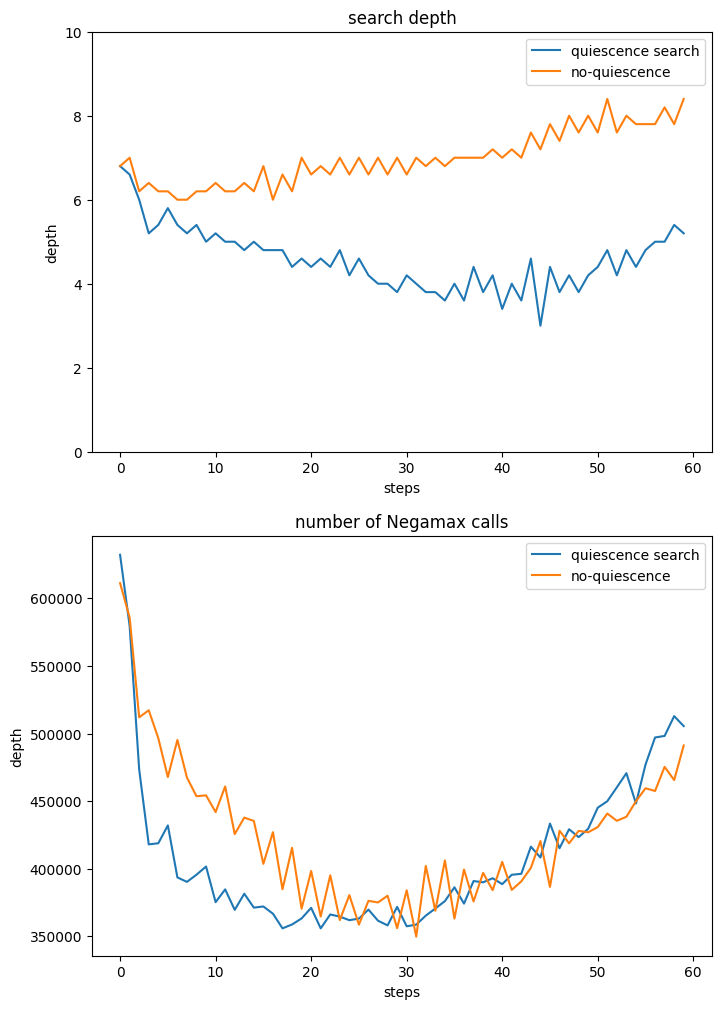
\includegraphics[totalheight=12cm]{image.png}
% \end{figure}

% We can find that the searching depth of non-quiescence solver is higher than quiescence solver, but the number of Negamax calls is similar.


\subsubsection{Experiments of different quiescence-search depth}

\begin{table}[!h]
  \centering
  \begin{tabular}{|c|c|c|c|}
    \diagbox{A}{B} & depth = 2 & depth = 4 & depth = 8 \\
    \hline
    depth = 6 & 51.5 / 48.5 & 48 / 52 &  51 / 49\\
    \hline
    depth = 0 & 37.5 / 62.5 & 41 / 59 &  40 / 60\\
  \end{tabular}
  
  \title{(score of A / score of B)}

  \title{score of different quiescence depth settings}
\end{table}


\subsection{Effect of Move Ordering}

Following experiments evaluate the result of ordering moves by comparing the different solvers as below
(configurations except move orvering are follow the standard configuration mentioned at \textbf{Implementation Detail}):
\begin{itemize}
  \item \textbf{standard}:
        The move-orderings performed as above
  \item \textbf{default-ordering}:
        Directly use the default order genrated by wakasagi engine(i.e. ordered by 將、士、象...).
  \item \textbf{random ordering}:
        Sort the moves with a randomly generated score of each move(control group)
\end{itemize}

Following is the performance of each group

\begin{table}[!h]
  \begin{tabular}{c|c|c|c}
      \diagbox{A}{B} & standard & default & random\\
      \hline
      standard & N/A & 15.5 / 4.5 & 14.5 / 5.5 \\
      \hline
      default & 4.5 / 15.5 & N/A & 4.5 / 15.5\\
      \hline
      random & 5.5 / 14.5 & 15.5 / 4.5 & N/A
  \end{tabular}  
\end{table}

% From the table above, we can find that the move-ordering is effective in improving the solver ability. Surprisingly, the random-ordering solver is stronger than the default-ordering solver.


\section{Appendix}

\subsubsection{Notations of SideDisScore}

\begin{align*}
  &SideDisScore_B(pos) =\\&\sum_{T} \frac{PV(T)}{2^{penalty(pos, T)}}\times \frac{\sum_{R,R.type = T} F_B(pos, R) + died(pos, Red, R)\times bound(T)}{initial(T)\times bound(T)}
\end{align*}


\begin{itemize}
  \item $initial(Red, T)$ is the number red pieces of type $T$ at the beginning of the game, i.e. $initial(\text{仕})=2, initial(\text{兵})=5$
  \item $died(Red, T)$ is the number of died red pieces of type $T$
  \item $bound(T)$ is the rough estimation of the upperbound of $F(pos, T)$, as the following table
  \begin{table}[!h]
    \begin{tabular}{|c|c|c|c|c|c|c|}
        帥 & 仕 & 相 & 俥 & 傌 & 炮 & 兵 \\
        \hline
        20$\times$5+10 &
        20+10$\times$ 2 &
        20$\times$3+10$\times$ 2 &
        20$\times$5+10$\times$ 2 &
        20$\times$7+10$\times$ 2 &
        20$\times$9 &
        20$\times$9+10$\times$5
    \end{tabular}
  \end{table}
  \item $penalty_B(pos, T) = 0$ if at least $2$ black pieces is strictly larger than $T$\\
  \item $penalty_B(pos, T) = 1$ if there's only one black piece strongly larger than $T$, and one piece equal to $T$\\
  \item $penalty_B(pos, T) = 2$ if there's only two equal black pieces and no stronger piece, or there's only one stronger piece and no equal piece.
  \item $penalty_B(pos, T) = 3$ if there's no stronger black piece, and strictly less than $2$ equal piece.
\end{itemize}

$2^{-penalty_B}$ will decrease the value for $T$ which is hard to capture for Black at current position, make it more focus on capturable pieces.

\subsubsection{Algorithm of MoveOrdering}
\begin{algorithm}
  \begin{algorithmic}
    \Procedure{MoveOrdering}{MovesList, depth, only\_critical}
    \If{depth <= 2}
      \State delete all Flipping moves from MovesList
    \EndIf
    \If{only\_critical is True}
      \State delete all non-capture and non-escape move from MoveList
    \EndIf
    \State MoveList $\gets$ Sort(MoveList, key(move) = EvalMove(move))
    \State \textbf{return} MoveList
    \EndProcedure
  \end{algorithmic}
\end{algorithm}

\subsubsection{Detail of Square Evaluation}

$SqEval(piece, sq)$ function is aimed to evaluate the advantage of $piece$ placing at $sq$.
More precisely, it evaluate the advantage by the mobility, information of adjancent/diagonal pieces of $sq$:
% Let $adjacent = {east, west, south, north}$ and $diagonal = {eastsouth, eastnorth, westsouth, westnorth}$


\begin{align*}
  SqEval(piece, sq) = Atk_{adj}(piece, sq) + 2\times Control(piece, sq) + Mobility(piece, sq)\\
  Atk_{adj}(piece, sq) = \sum_{P_{adj}\in adjacent\_pieces(sq)} can\_capture(piece, P_{adj})\times PV[P_{adj}]\\
  Control(piece, sq) = \sum_{P_{diag}\in diagonal\_pieces(sq)} can\_capture(piece, P_{diag})\times PV[P_{diag}]\\
  Mobility(piece, sq) = \sum_{adj\in adjacent(sq)} can\_goto(piece, adj)
\end{align*}

The boolean function $can\_goto(P, sq)$ return true if the piece $P$ can move to $sq$, i.e. there's empty or piece can capture the piece there.\\
$can\_capture(P_1, P_2)$ return true if $P_1, P_2$ not at the same side, and $P_1$ can capture $P2$



\subsubsection{Detail of History Heuristic}
The weight of history heuristic as follow

\begin{algorithm}
  \begin{algorithmic}
    \Procedure{update\_cut\_move}{move, depth}
        \State history[move] += $2 \times depth$
        \If{history[move] $\ge bound_{history}$}
          \State decrease()
        \EndIf
    \EndProcedure

    \Procedure{update\_optimal\_move}{move, depth}
        \State history[move] += $depth^2$
        \If{history[move] $\ge bound_{history}$}
          \State decrease()
        \EndIf
    \EndProcedure

    \Procedure{decrease}{}
      \For{move $\in$ any moves in the board}
        \State history[move]$ = \frac{\text{history[move]}}{2}$
      \EndFor
    \EndProcedure

  \end{algorithmic}
\end{algorithm}



\end{document}